\section{全景池的用途}

全景池覆盖 50 个 Atlas/AIDC 相关节点，包含上市公司、海外公司、私营/不可投资节点、下游需求锚、低纯度公司和公开信息不可得节点。它的目的不是制造 50 只受益股，而是确保每个物理环节都有状态、证据、估值处置和下一验证路径。对没有平台关系或经济性证据的公司，分类为卫星/观察；对海外、私有或缺少上市标的的节点，保留在技术图谱但不进入 A 股目标价。

\begin{exhibitbox}[Atlas 950/AIDC 相关节点全景表（50 个节点）]
\scriptsize
\setlength{\tabcolsep}{1.5pt}
\begin{longtable}{L{1.0cm}L{2.2cm}L{2.5cm}L{3.0cm}L{2.2cm}L{2.0cm}L{1.8cm}}
\toprule
\textbf{ID} & \textbf{模块} & \textbf{子环节} & \textbf{节点/公司} & \textbf{代码/市场} & \textbf{分类} & \textbf{证据状态}\\
\midrule
\endhead
FC001 & 算力与需求锚 & AI 加速器 & 华为昇腾 950DT & not listed & 需求锚 & 官方路线图\\
FC002 & 算力与需求锚 & 超节点平台 & 华为 Atlas 950 SuperPoD & not listed & 需求锚 & 官方实物披露\\
FC003 & 算力与需求锚 & 加速器竞品 & 英伟达 Rubin NVL 平台 & NVDA.US & 范围外参照 & 官方竞品参照\\
FC004 & 算力与需求锚 & 加速器竞品 & AMD Instinct/UALink 生态 & AMD.US & 范围外参照 & 官方生态参照\\
FC005 & 算力与需求锚 & 模型训练应用 & 科大讯飞 & 002230.SZ & 核心估值 & 官方披露\\
FC006 & 算力与需求锚 & 国产加速器竞品 & 寒武纪/海光/摩尔线程 & 688256.SH / 688041.SH / 688795.SH & 范围外参照 & 官方产品参照\\
FC007 & 服务器/整柜 & 超节点集成 & 华为计算产品线 & not listed & 需求锚 & 官方披露\\
FC008 & 服务器/整柜 & 服务器生态 & 拓维信息/兆瀚 & 002261.SZ & 卫星观察 & 官方披露\\
FC009 & 服务器/整柜 & 服务器生态 & 神州数码/鲲泰 & 000034.SZ & 卫星观察 & 官方披露\\
FC010 & 服务器/整柜 & 服务器 OEM & 超聚变 & not listed & 范围外参照 & 行业参照\\
FC011 & 服务器/整柜 & 服务器 OEM 竞品 & 浪潮信息 & 000977.SZ & 卫星观察 & 官方产品能力\\
FC012 & 服务器/整柜 & 传闻 ODM 映射 & 四川长虹 & 600839.SH & 范围外参照 & 官方否认\\
FC013 & 供配电 & 综合供电 & 华为数字能源 & not listed & 需求锚 & 公司能力\\
FC014 & 供配电 & UPS/基础设施 & 科华数据 & 002335.SZ & 卫星观察 & 官方披露\\
FC015 & 供配电 & HVDC 供电 & 中恒电气 & 002364.SZ & 卫星观察 & 官方产品能力\\
FC016 & 供配电 & 变压器/磁性元件 & 伊戈尔 & 002922.SZ & 卫星观察 & 官方产品能力\\
FC017 & 供配电 & UPS & 科士达 & 002518.SZ & 卫星观察 & 官方产品能力\\
FC018 & 供配电 & 母线/变压器/备电 & Atlas 专属电气 BOM & not available & 不可得 & 未找到\\
FC019 & 液冷/热管理 & 端到端液冷 & 申菱环境 & 301018.SZ & 核心估值 & 官方披露\\
FC020 & 液冷/热管理 & 端到端液冷 & 英维克 & 002837.SZ & 核心估值 & 官方披露\\
FC021 & 液冷/热管理 & 工业液冷 & 同飞股份 & 300990.SZ & 卫星观察 & 官方产品能力\\
FC022 & 液冷/热管理 & 液冷系统 & 高澜股份 & 300499.SZ & 卫星观察 & 官方产品能力\\
FC023 & 液冷/热管理 & 液冷连接器 & 航天电器 & 002025.SZ & 卫星观察 & 官方产品能力\\
FC024 & 液冷/热管理 & 冷却液/泵阀 & Atlas 专属流体子系统 & not available & 不可得 & 未找到\\
FC025 & 光网络/互联 & Scale-up 互联 & 华为 UnifiedBus/灵衢 & not listed & 需求锚 & 官方披露\\
FC026 & 光网络/互联 & 光交换/OCS & 华为跨柜光互联 & not listed & 需求锚 & 官方架构披露\\
FC027 & 光网络/互联 & 光模块/光引擎 & 华工科技 & 000988.SZ & 核心估值 & 官方产品/交付\\
FC028 & 光网络/互联 & 光模块 & 光迅科技 & 002281.SZ & 卫星观察 & 官方产品能力\\
FC029 & 光网络/互联 & 光器件 & 天孚通信/光库科技 & 300394.SZ / 300620.SZ & 卫星观察 & 官方产品能力\\
FC030 & 光网络/互联 & 高速铜缆 & 沃尔核材/兆龙互连 & 002130.SZ / 300913.SZ & 卫星观察 & 官方产品能力\\
FC031 & 光网络/互联 & 高速连接器 & 鼎通科技 & 688668.SH & 卫星观察 & 官方产品能力\\
FC032 & 光网络/互联 & 交换/NIC 芯片 & 华为自研交换/NIC 栈 & not listed & 不可得 & 仅系统归属推断\\
FC033 & 存储/内存 & 类 HBM 内存 & 华为 HiZQ 2.0 & not listed & 需求锚 & 官方路线图\\
FC034 & 存储/内存 & DRAM 晶圆制造 & 国产 DRAM 制造映射 & not available & 不可得 & 传闻/未确认\\
FC035 & 存储/内存 & 内存接口 & 澜起科技 & 688008.SH & 卫星观察 & 官方产品能力\\
FC036 & 存储/内存 & SPD/EEPROM & 聚辰股份 & 688123.SH & 卫星观察 & 官方产品能力\\
FC037 & 存储/内存 & 企业级 SSD & 佰维存储/江波龙/德明利 & 688525.SH / 301308.SZ / 001309.SZ & 卫星观察 & 官方产品能力\\
FC038 & PCB/连接 & 高速 CCL & 生益科技 & 600183.SH & 卫星观察 & 官方产品能力\\
FC039 & PCB/连接 & 高速 PCB & 深南电路 & 002916.SZ & 卫星观察 & 官方产品能力\\
FC040 & PCB/连接 & 高速 PCB & 沪电股份 & 002463.SZ & 卫星观察 & 官方产品能力\\
FC041 & PCB/连接 & 高密度 PCB & 胜宏科技 & 300476.SZ & 卫星观察 & 官方产品能力\\
FC042 & PCB/连接 & ABF 载板/PCB & 广合科技 & 002436.SZ & 卫星观察 & 官方产品能力\\
FC043 & PCB/连接 & 探针卡 & 强一股份 & 688809.SH & 卫星观察 & 公司未确认\\
FC044 & IDC/应用 & 云平台 & 华为云 & not listed & 需求锚 & 官方需求锚\\
FC045 & IDC/应用 & 电信运营商 & 中国移动 & 600941.SH / 00941.HK & 需求锚 & 官方需求锚\\
FC046 & IDC/应用 & 电信运营商 & 中国电信 & 601728.SH / 00728.HK & 需求锚 & 官方需求锚\\
FC047 & IDC/应用 & 电信运营商 & 中国联通 & 600050.SH / 00762.HK & 需求锚 & 官方需求锚\\
FC048 & IDC/应用 & 模型应用 & 科大讯飞 & 002230.SZ & 核心估值 & 官方披露\\
FC049 & IDC/应用 & IDC/托管 & 国内 IDC 运营商 & 300738.SZ / 300442.SZ / 600845.SH & 卫星观察 & 官方产能参照\\
FC050 & IDC/应用 & 政策/公共算力 & 国家及地方智算项目 & not applicable & 需求锚 & 官方政策\\
\bottomrule
\end{longtable}
\sourcenote{50 节点全链条证据池。分类只表示研究处置，不表示 Atlas 950 供货或投资评级。}
\end{exhibitbox}


\begin{figure}[htbp]
\centering
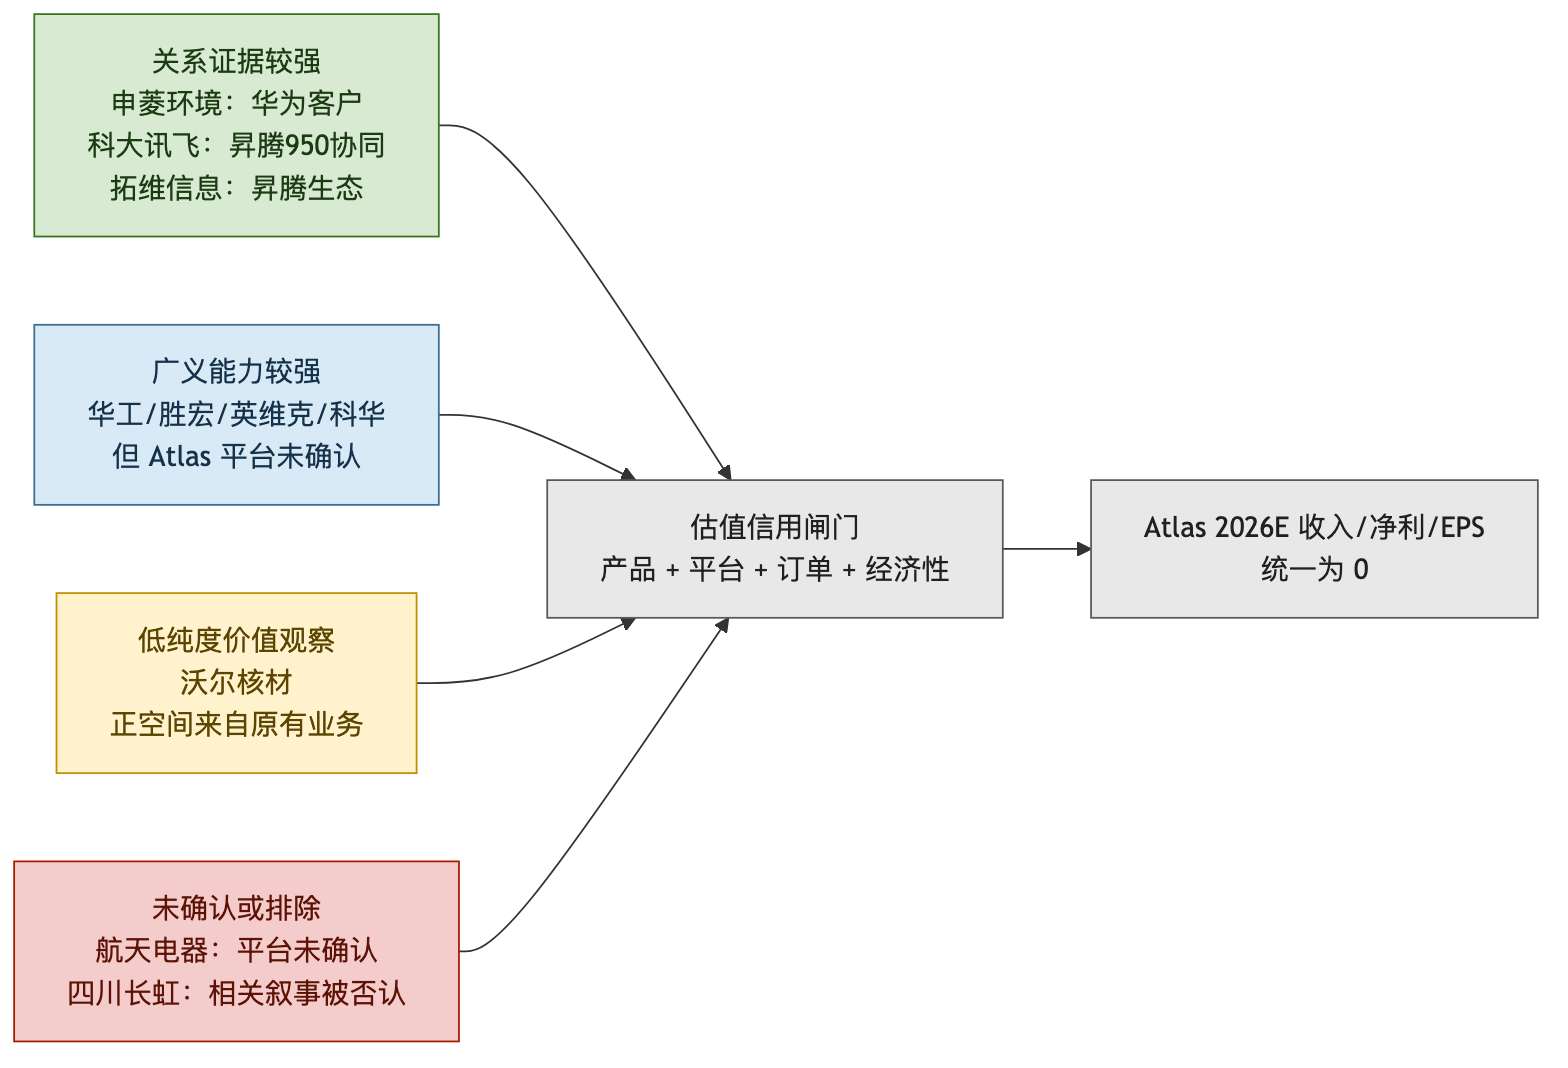
\includegraphics[width=0.96\textwidth]{exhibits/company_evidence_heatmap.png}
\caption{公司关系证据、广义能力与 Atlas 盈利信用分层}
\sourcenote{公司年报、客户链审计与公司级分类对账。颜色表示研究证据状态，不表示收益率预测。}
\end{figure}

\section{三类池与一个排除池}

\textbf{关系验证池}包括申菱环境、科大讯飞和拓维信息。它们分别代表冷却客户关系、950 下游协同和昇腾生态，但没有 Atlas 专属盈利闭环。\textbf{基本面估值池}包括 12 个拥有正权重原始卖方预测、可复算目标的公司，评价的是更广义业务。\textbf{能力卫星池}包括光器件、PCB/CCL、连接器、供电和液冷公司，只有在平台点名、认证和订单出现后才升级；航天电器位于该池，已确认高速背板/液冷连接器能力，但未确认华为/950 客户关系。

\textbf{排除池}包括两类：一是明确否认市场叙事的四川长虹；二是投资者提问但公司没有确认的昇腾 950 探针卡/HBM 等关系。排除不是永久结论，若出现新的一级证据可以重新进入审计；在此之前不得以“互动平台提问”作为供应商证据。

\begin{exhibitbox}[12 家公司三维分类对账]
\begin{longtable}{L{1.35cm}L{1.8cm}L{3.25cm}L{2.25cm}L{2.15cm}L{3.0cm}}
\toprule
\textbf{代码} & \textbf{公司} & \textbf{Atlas 关系证据} & \textbf{广义估值} & \textbf{研究动作} & \textbf{分歧原因}\\
\midrule
\endhead
000034 & 神州数码 & 华为/昇腾生态；Atlas 未确认 & 可估值 & 观察 & 生态不等于订单；现金周转决定倍数\\
000988 & 华工科技 & AI 光连接能力；Atlas 未确认 & 可估值 & 等待平台订单 & 全球 AI 盈利与 Atlas 卫星身份并存\\
600183 & 生益科技 & AI 材料能力；Atlas 规格未知 & 可估值 & 避免追高 & 按 CCL 盈利估值，不给平台份额\\
002916 & 深南电路 & AI PCB 能力；Atlas 认证未知 & 可估值 & 回调验证 & 只计已披露 AI 业务\\
002463 & 沪电股份 & AI PCB 能力；客户分配未知 & 可估值 & 回调验证 & 卫星节点但有独立盈利\\
300476 & 胜宏科技 & 全球 AI PCB；Atlas 未确认 & 可估值 & 选择性观察 & 正空间来自全球 AI，不来自链纯度\\
002837 & 英维克 & 液冷能力；华为分配未确认 & 可估值 & 等待毛利恢复 & 产品能力支持 AIDC，专属信用为零\\
301018 & 申菱环境 & 华为客户强；Atlas 订单未确认 & 可估值 & 最高关系观察 & 关系最强，估值仅计广义数据服务\\
002335 & 科华数据 & 昇腾邻近项目；Atlas 未确认 & 可估值 & 等待估值回落 & 项目能力成立，平台专属性不足\\
002130 & 沃尔核材 & 高速连接能力；Atlas 未确认 & 可估值 & 低纯度价值卫星 & 正空间仅依赖原有业务\\
002230 & 科大讯飞 & 昇腾 950 协同；非硬件供应商 & 下游可估值 & 事件验证 & 需求锚可估值，不等于硬件订单\\
002025 & 航天电器 & 产品能力；平台关系未确认 & 可估值 & 关系未确认观察 & 问答只确认产品，不确认客户\\
\bottomrule
\end{longtable}
\sourcenote{公司级对账以代码去重；关系强度、广义业务估值资格和研究动作是三个独立维度。节点级全景表可重复同一公司，但不得改变本表的公司级结论。}
\end{exhibitbox}


三维对账解决了节点表中同一公司可能重复、但公司结论只能有一个的问题。申菱环境的关系证据最强，却只按广义数据服务估值；科大讯飞是需求锚而非硬件供应商；沃尔核材和胜宏科技存在正目标空间，却不能被升级为华为 Atlas 核心。关系、估值资格与动作因此不再由单一“核心/卫星”标签替代。

\section{下一条验证路径}

算力/HBM 节点需要制造、封装、良率与量产来源；整柜节点需要 OEM/ODM、柜型、订单和服务边界；光互联需要端口数、速率、形态与供应商；PCB/连接器需要平台规格、认证、良率与 ASP；供电/液冷需要系统 MW、kW/柜、CDU/冷板/快接数量与订单；IDC/应用需要客户、站点、验收、利用率和计费。全景池每一行都指向这些可执行问题，而不是用泛化“受益逻辑”收尾。
